\chapter{Underwater Robotics}
\section{Introduction}
Although robots can roam around the ground or even fly, most of the Earth's surface is covered in water. This immediately highlights the need for robots to become capable of handling such environments; this is the objetive of \textit{underwater robotics}. Similarly as in the case of aerial robotis, underwater robots can be classified as:
\begin{itemize}
    \item \textit{Remotely Operated Vehicles}, which are connected by a tether to an operator or surface ship.
    \item \textit{Autonomous Underwater Vehicles}.
    \item \textit{Unmanned Underwater Vehicles}.
    \item \textit{Underwater Vehicle-Manipulator Systems}.
\end{itemize}
In general, design of underwater robots is more difficult than ground or aerial ones:
\begin{itemize}
    \item GPS doesn't work underwater. \textit{Sonars} are employed.
    \item There is no single proprioceptive sensor for localization.
    \item Visibility is often scarse.
    \item Sonars are noisy sensors.
    \item The allocation matrix is very difficult to obtain, due to the highly nonlinear relationship between force/moment acting along the body and the control inputs.
\end{itemize}
\section{Dynamic Model}
The dynamic model is fairly similar to the one of an UAV, although the gravity term is missing and requires special care. 
\begin{figure}[htbp!]
    \begin{minipage}{0.6\textwidth}
        \centering
        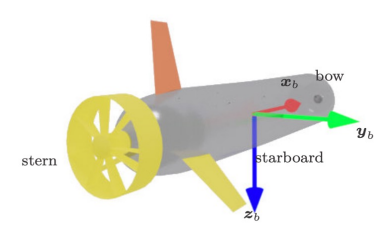
\includegraphics[width=1\linewidth]{Images/body_underwater.png}
        \caption{Underwater robot's\\ body frame.}    
    \end{minipage}
    \hfill               
    \begin{minipage}{0.4\textwidth}
        Another difference stands in the name of the angles used to represent angular motion; in underwater robotics, Roll-Pitch-Yaw angles are substituted by \textit{Surge-Sway-Heave} angles.
        \begin{itemize}
            \item \textit{Surge} along the $x$-axis.
            \item \textit{Sway} along the $y$-axis.
            \item \textit{Heave} along the $z$-axis.
        \end{itemize}
    \end{minipage}
\end{figure}
The dynamics model is then given.
\begin{definition}
    \textit{Underwater Robot's Dynamic Model}:
    \begin{gather}\label{underwater_robot_dyn_mod}
        \begin{bmatrix}
            mI_{3} & 0_3 \\
            0_3 & J_{b}
        \end{bmatrix}
        \begin{bmatrix}
            \ddot{p}_{b}^{b}\\
            \dot{\omega}_{b}^{b}
        \end{bmatrix}+
        \begin{bmatrix}
            mS(\omega_{b}^{b}) & 0\\
            0 & S(\omega_{b}^{b})J_b
        \end{bmatrix}=
        \begin{bmatrix}
            f^b \\ \tau^b
        \end{bmatrix}\\
        \dot{R}_b=R_bS(\omega_b^b)
    \end{gather}
\end{definition}
\subsection{Working in water: currents, buoyancy and added inertia}
Underwater robots have another difficulty to overcome: to achieve their movement, they also have to push the water in front of them. This implies:
\begin{itemize}
    \item An added inertia has to be considered, since the water applies reaction forces on the robot's body. This is the \textit{Added Mass Contribution}, which is a function of the body's geometry. This also implies that its associated mass matrix is not necessarily positive-definite or symmetric. 
    \item The presence of fluid causes drag and lift on the body. These effect are often lumped into a constant damping term.
\end{itemize}
Other significant contributions to the robot's dynamics are given by the presence of wind and currents. In particular, currents, $v_c$, can be assumed as irrotational and constant, then added to the model before computing the Coriolis, centripetal and damping terms:
\begin{gather*}
    v_r=\begin{bmatrix}
        \dot{p}_b^b\\ \omega_b^b
    \end{bmatrix}-R_b^Tv_c
\end{gather*}
Finally, the robot's buoyancy has to be taken into account. Notice that this is a \textit{hydrostatic} effect, meaning that it does not depend on the robot's speed. Define $b=\rho\Delta\|g\|$ to be the buoyancy force exerted on the body, which is submerged in a liquid of density $\rho$ for a certain amount $\Delta$ of its own volume. Then, the resulting wrench acting on the body expressed in the world-frame is:
\begin{gather*}
    g_{rb}^b=-
    \begin{bmatrix}
        f_g^b+f_b^b\\
        S(r_c^b)f_g^b+S(r_b^b)f_b^b
    \end{bmatrix}
\end{gather*}
Which is taken into account in the following UUV model:
\begin{definition}
    \textit{UUV Dynamic Model with buoyancy and current contribution in World-Frame:}
    \begin{gather}
        M_v
        \begin{bmatrix}
            \ddot{p}_b^b\\ \dot{\omega}_b^b
        \end{bmatrix}+(C_v+D_{RB})
        \begin{bmatrix}
            \dot{p}_b^b\\ \omega_b^b
        \end{bmatrix}+g_{rb}^b=\tau_v-\tau_{v,c}\\
        M_v=M_v^T,\quad D_{RB}>0,\quad C_v=-C_v^T
    \end{gather}
    Where $\tau_v$ is often taken to be:
    \begin{equation}
        \tau_v=B_vu_v
    \end{equation}
    Where $B_v$ is the \textit{Thrusters Control Matrix}.
\end{definition}
The model can be written with respect to the body-frame by finding a set of parameters $\theta_v$ for which it is linear. In that case, a regressor matrix can be found such that:
\begin{equation*}
    \phi_v\theta_v=\tau_v
\end{equation*}
It is useful to separate the \textit{persistent dynamics}, the one which affects the robot even when it is still, from the general dynamics; this results in the following model.
\begin{definition}
    \textit{UUV Dynamic Model with buoyancy and current contribution in Body-Frame:}
    \begin{gather}
        M_v
        \begin{bmatrix}
            \ddot{p}_b^b\\ \dot{\omega}_b^b
        \end{bmatrix}+(C_v+D_{RB})
        \begin{bmatrix}
            \dot{p}_b^b\\ \omega_b^b
        \end{bmatrix}+g_{rb}^b+
        \phi_{v,p}\theta_{v,p}\\
        \phi_{v,p}\theta_{v,p}=\phi_{v,r}\theta_{v,r}+\phi_{v,c}\theta_{v,c}
    \end{gather}
    Where $\phi_{v,r}$ is the regressor of the \textit{restoring} forces (buoyancy and gravity), $\phi_{v,c}\theta_{v,c}$ is the one referred to currents. If the currents are considered as constant and expressed in the world-frame, then:
    \begin{gather*}
        \phi_{v,p}=\begin{bmatrix}
            R_b^Te_3 & 0_3 & R_b^T & 0_3 \\
            0_3^T & S(R_b^Te_3) & 0_3 & R_b^T
        \end{bmatrix}
    \end{gather*}
    Otherwise:
    \begin{gather*}
        \phi_{v,p}=\begin{bmatrix}
            R_b^Te_3 & 0_3 & I_3 & 0_3 \\
            0_3^T & S(R_b^Te_3) & 0_3 & I_3
        \end{bmatrix}
    \end{gather*}
\end{definition}
Restoring forces pose a challenge both in terms of modeling and control, especially for large UUVs. In particular, restoring forces are well expressed in the body-frame, meanwhile currents are better expressed in the world-frame, this adds a layer of complexity to the modeling. Adaptive Controllers are best suited for underwater applications.